\section{Task 1}

\subsection{Overview of Horner's method}

Horner's method efficiently evaluates a polynomial \( P(x) \) at a given point \( x \). Its main advantage is to reduce the required operations, lowering computational complexity from \( O(n^2) \) to \( O(n) \), where \( n \) is the polynomial degree.

The algorithm's basic idea can be expressed recursively as follows:
\[
P(x) = a_n + x(a_{n-1} + x(a_{n-2} + \dots + x(a_1 + x a_0)))
\]
Evaluation requires only \( n \) multiplications and \( n \) additions, substantially reducing computation time for high-degree polynomials.

Tests used polynomial sizes from 100 to 5000 in steps of 100. For each degree, 100 different polynomials were sampled. Each polynomial was evaluated using Horner's method and the standard method; the measured runtimes were then averaged.

\subsection{Results and conclusions}

The two types of plots below illustrate the experimental results:

\begin{center}
\begin{minipage}{0.45\textwidth}
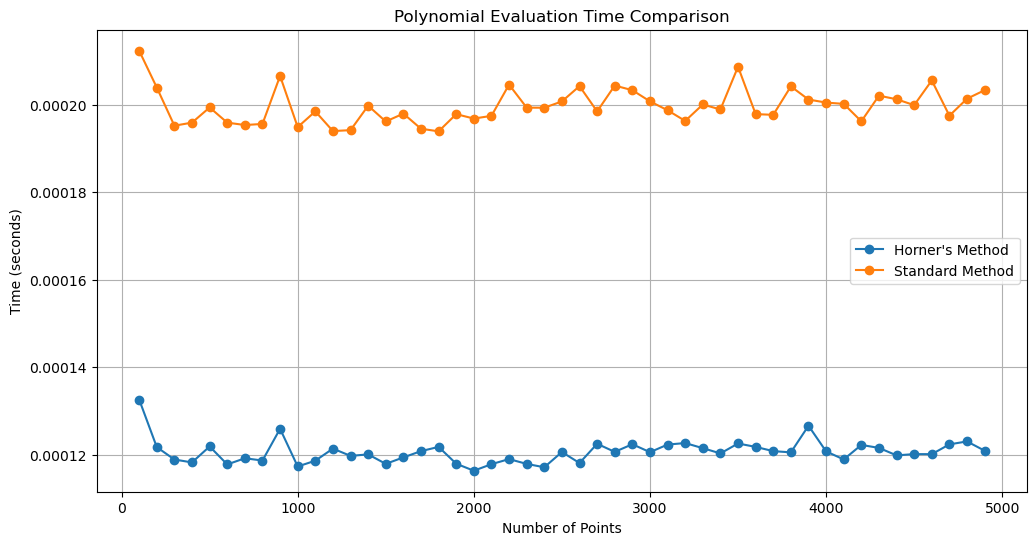
\includegraphics[width=\textwidth]{figures/task-1/horner_1.png}
\end{minipage}
\begin{minipage}{0.45\textwidth}
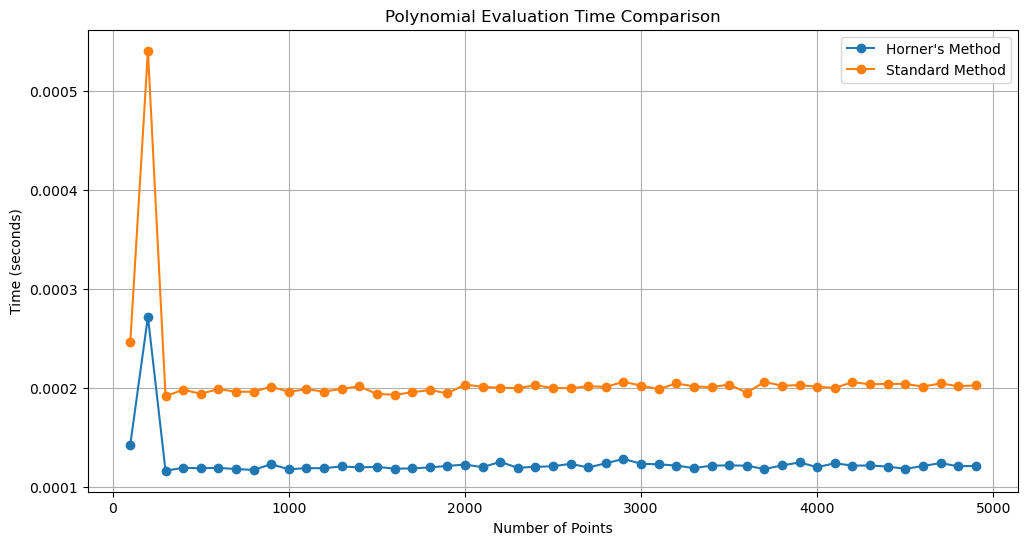
\includegraphics[width=\textwidth]{figures/task-1/horner_2.png}
\end{minipage}
\end{center}

\textbf{Conclusions:}
\begin{itemize}
    \item \textbf{Speed improvement:} Horner's method gives an average speed improvement of \( 1.64 \pm 0.04 \), consistent with expectations from reduced computational complexity.
    \item \textbf{Unexpected runtime spikes:} Some trials showed a significant runtime increase for an individual polynomial. This did not correlate with coefficient magnitude or polynomial size; its cause is unknown.
    \item \textbf{Scalability:} Horner's method scales well to high polynomial degrees, maintaining stable computation times compared with the classical algorithm.
\end{itemize}

